\section{Method Comparison}
In the following sections, the methods explained previously are going to be compared for multiple examples. First, the integer-order algorithms and ABM for some integer-order systems and then a comparison of the fractional algorithms is performed. 

\subsection{Integer models}
Ensuing, four examples for integer systems of ODEs are presented, in order to compare ABM, Euler and RK4.
\subsubsection{Chaotic Financial System}
Recall the example \ref{ex:finance}. This system will now be compared with the Adams-Bashforth-Moulton predictor-corrector algorithm for an integer system of ODEs. The results of this simulation are presented in figure \ref{fig:comparFinanceX}.

\begin{figure}[H]
    \centering
    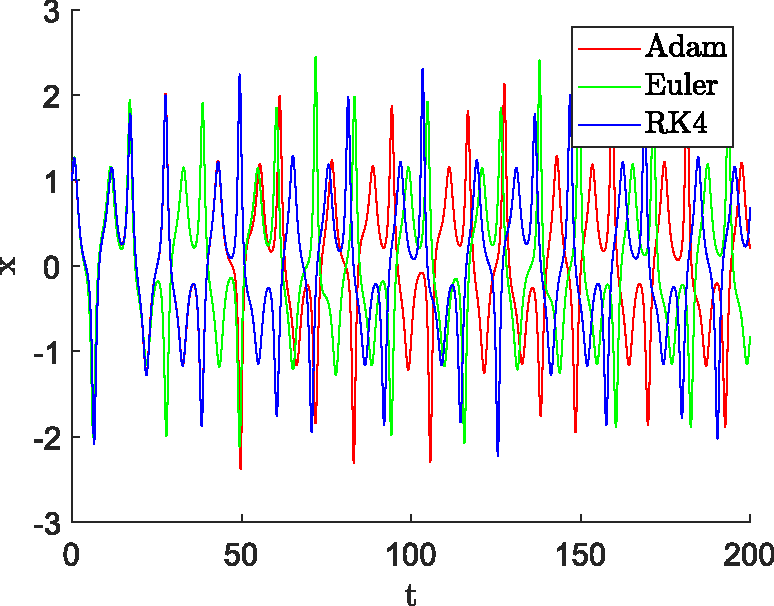
\includegraphics[scale=0.5]{files/adm_euler_rk4_x.pdf}
    \caption{}
    \label{fig:comparFinanceX}
\end{figure}



\subsubsection{Thomas' Cyclically Symmetric Attractor}
This system was originally proposed by R. Thomas in \cite{thomas1999deterministic}. It describes a deterministic fractional Brownian motion, this system can be used to model auto-catalytic chemical reactions, ecology and evolution systems. The parameter $b$ represents the frictional damping for a particle moving in a 3D labyrinth \cite{sprott2007labyrinth}. This dynamic system is given by
\begin{equation}
    \begin{cases}
        x'=\sin(y)-bx&\\
        y'=\sin(z)-by&\\
        z'=\sin(x)-bz&\\
    \end{cases}
\end{equation}

The following simulations were performed with initial conditions $(x_0,\,y_0,\,z_0)=(0,\,0.1,\,0)$ and $b=0.18$; each figure shows the state variables through time, where it was use three different numeric methods to solve the system. For the ABM predictor-corrector, $\alpha=1$ since it is a system of integer ordinary differential equations
\begin{figure}[H]
\centering
\begin{subfigure}[ht]{0.3\textwidth}
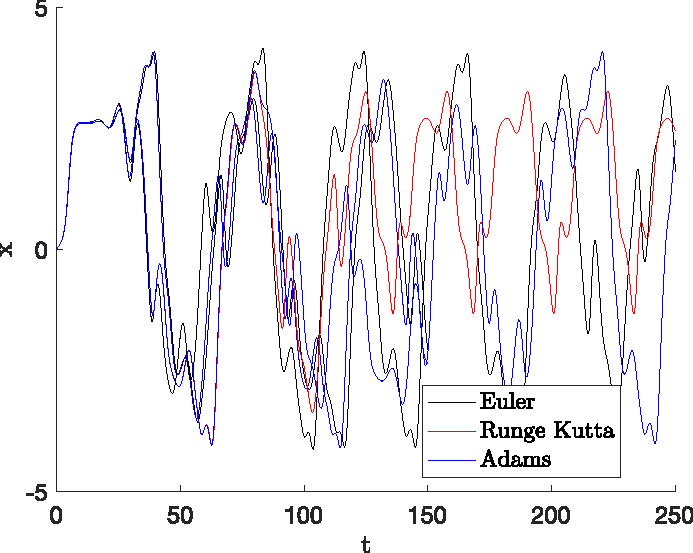
\includegraphics[scale=0.33]{files/ThomasXvsT.pdf}
\end{subfigure}
\begin{subfigure}[ht]{0.3\textwidth}
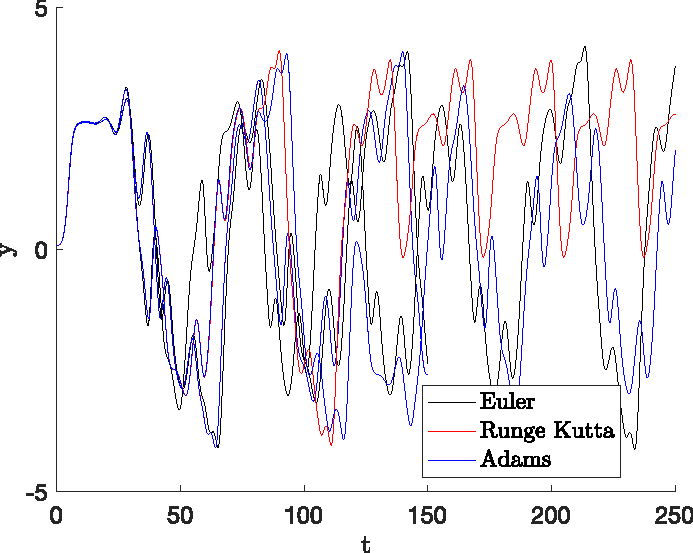
\includegraphics[scale=0.33]{files/ThomasYvsT.pdf}
\end{subfigure}
\begin{subfigure}[ht]{0.3\textwidth}
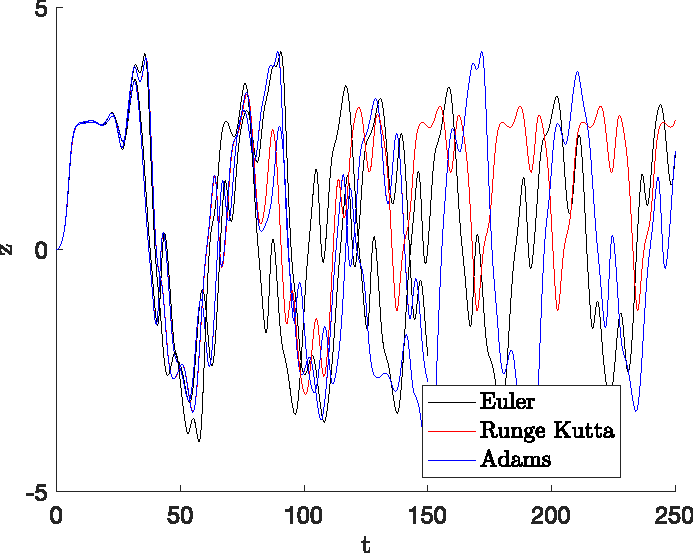
\includegraphics[scale=0.33]{files/ThomasZvsT.pdf}
\end{subfigure}
\caption{}
\label{fig:thomasExample}
\end{figure}

The 3D portrait of the Thomas' system is shown in figure \ref{fig:thomas3d}.
\begin{figure}[H]
    \centering
    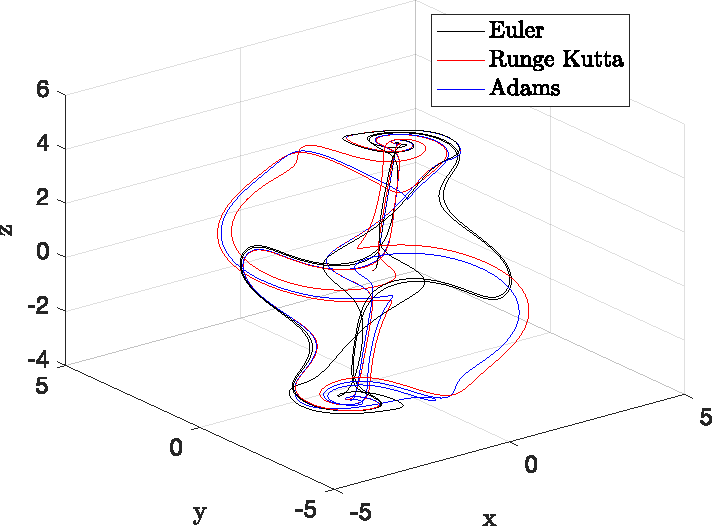
\includegraphics[scale=0.6]{files/3DThomas.pdf}
    \caption{3D phase portrait for the Thomas' system.}
    \label{fig:thomas3d}
\end{figure}

In order to compare Euler, RK4 and ABM methods, we present the results in figure \ref{fig:thomasExample}. It can be easily seen that in the beginning of the simulation the three solutions has similar behavior. Lately, the three solutions diverge compared to each other, but RK4 and ABM, stay more time with similar behavior. The discrepancies are possible due to the different calculations that each method needs, carrying his own errors. Other important fact to have into account, is that we are simulating a chaotic system, so small changes generate big differences in the future.


\subsubsection{Langford (Aizawa) Attractor}
The following set of differential equations were proposed by W. F. Langford in \cite{langford1984numerical}. This system is often called the Aizawa Attractor. 
\begin{equation}
    \begin{cases}
        x'=(z-\beta)x-\omega y&\\
        y'=\omega x+(z-\beta)y&\\
        z'=\lambda+\alpha z-\dfrac{z^3}{3}-(x^2+y^2)(1+\rho z)+\epsilon zx^3&\\
    \end{cases}
\end{equation}
The following simulations were performed with initial conditions $(x_0,\,y_0,\,z_0)=(0.1,\,0,\,0)$ and $\alpha=0.95$, $\beta=0.7$, $\lambda=0.6$, $\omega=3.5$, $\rho=0.25$ and $\epsilon=0.1$; each figure shows the state variables through time, where it was use three different numeric methods to solve the system. For the ABM predictor-corrector, $\alpha=1$ since it is a system of integer ordinary differential equations.
\begin{figure}[H]
\centering
\begin{subfigure}[b]{0.4\textwidth}
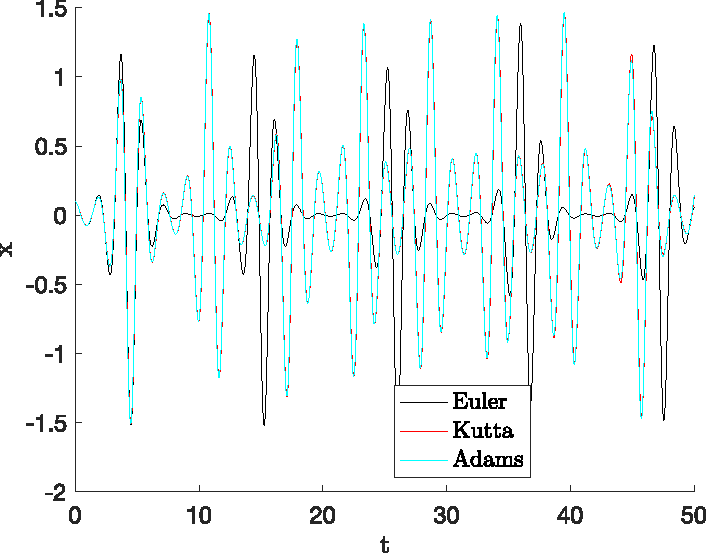
\includegraphics[scale=0.45]{files/AizawaXvsT.pdf}
\end{subfigure}
\hspace{1.5cm}
\begin{subfigure}[b]{0.4\textwidth}
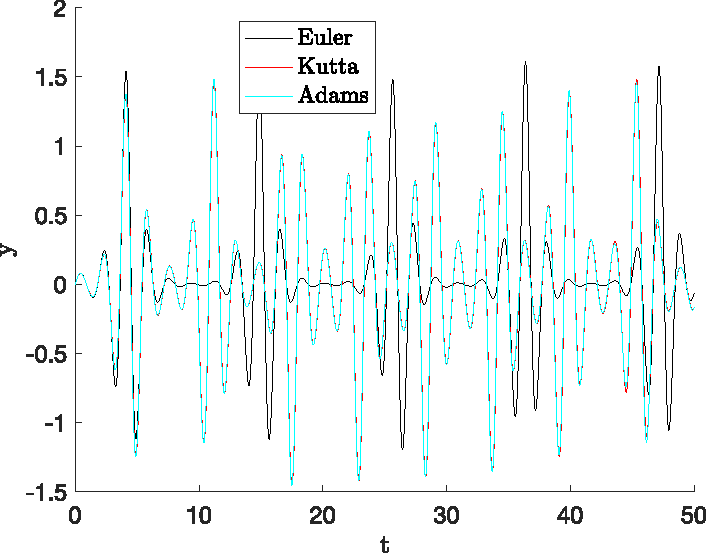
\includegraphics[scale=0.45]{files/AizawaYvsT.pdf}
\end{subfigure}
\vskip\baselineskip
\begin{subfigure}[b]{0.4\textwidth}
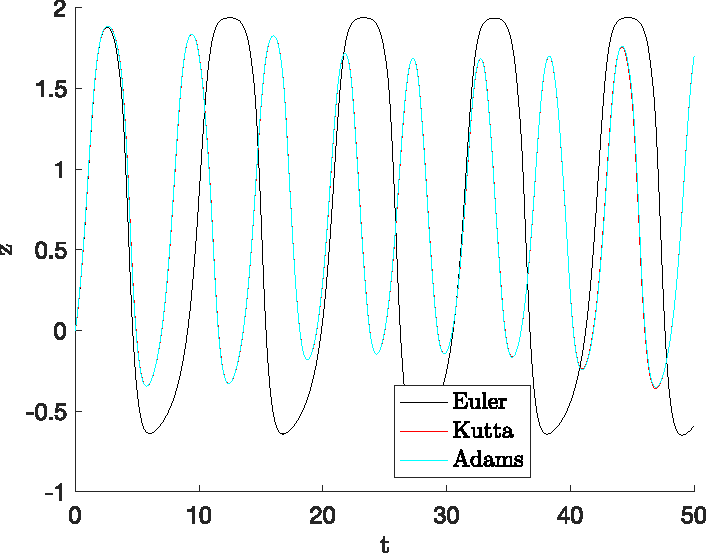
\includegraphics[scale=0.45]{files/AizawaZvsT.pdf}
\end{subfigure}
\caption{State variables response in time.}
\label{fig:aizawaExample}
\end{figure}

\begin{figure}[H]
    \centering
    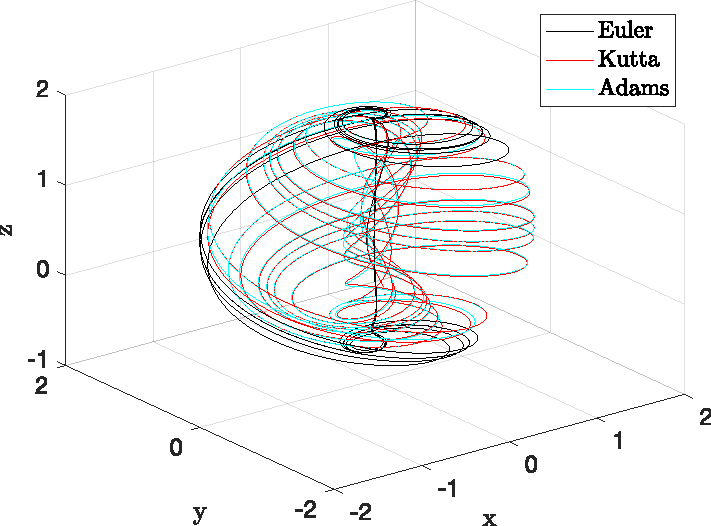
\includegraphics[scale=0.5]{files/3DIntegerAizawa.pdf}
    \caption{3D phase portrait for the Aizawa's system.}
    \label{fig:aizawa3d}
\end{figure}

With the Aizawa's systems occurs something similar with what we have already discussed in the previous section, with the difference that ABM and RK4 stayed together, overlapping the signals during the simulation except in the time series of the state variable $y$ approximately in the time 45, where RK4 has a lower peak proving that, effectively, RK4 and ABM overlap.

\subsubsection{Integer order systems}\label{subsec:int_ord}

Solve the following set of differential equations, using Euler, RK4, ABM and Decomposition, with the initial conditions $x(0) = 1, y(0) = -1$.

\begin{equation}
    \begin{cases}
        x'= y&\\
        y'= 2x - y&\\
    \end{cases}
\end{equation}

Carrying out some analytic operations, the exact solution is given by:

\begin{equation}
    \begin{cases}
        x = \dfrac{1}{3}e^{-2t}(e^{3t}+2)&\vspace{2mm}\\
        y = 
        \dfrac{1}{3}e^{-2t}(e^{3t}-4)&\\
    \end{cases}
\end{equation}

In the figure \ref{fig:int_todos} is compare the exact solution with decomposition, RK4, Euler and ABM.

\begin{figure}[H]
    \centering
    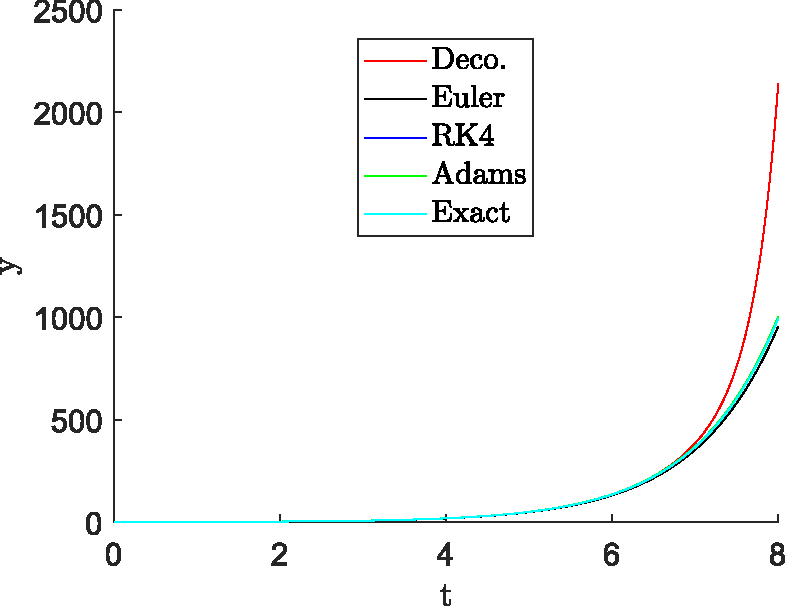
\includegraphics[scale=0.5]{files/int_todos.pdf}
    \caption{Results using different methods.}
    \label{fig:int_todos}
\end{figure}

It can be easily seen that during the simulation all the methods overlap the exact solution, except Decomposition (red signal) that in the time seven, it starts increase more than the other ones, because even though this method gives an analytical solution, it use a polynomial with infinite terms, so it´s necessary to truncate it in some point and then is when it diverges compare with the exact solution.

\subsection{Fractional models}
Subsequent, it is presented some examples SOMEEEEEEEEEEEEEEEEEEEEEEEEEEEEEEEEEEEEEEEEEE OR ONE??????????????????????????????????????????????????????????????????? to compare the fractional methods with the exact solution, i.e Decomposition and ABM.

\subsubsection{ABM and decomposition}

In order to compare Decomposition and ABM, it was solved the following the fractional initial value problem, with $y(0) = 1$ and $y'(0)=0$. Notice that is the same example present on each method (for ABM example \ref{ex:adam} and for Decomposition \ref{ex:deco}). 
\begin{equation}
    \mathcal{D}_c^{1.25}y(t)=-y(t)
\end{equation}
Carrying out some analytic operations, the exact solution is given by
\begin{equation}
    y(t) = E_{1.25,\,1}(-t^{1.25})=\sum_{k=0}^{\infty}\dfrac{(-1)^kt^{1.25k}}{\Gamma(1.25k +1)}
\end{equation}

In order to obtain a numerical solution Decomposition was performed with $15$ polynomial terms and ABM with a step-size $h=0.01$. Analyzing the figure \ref{fig:abm_decomp}, it can easily seen that it happen the same as in the comparison of the methods, in the previous section, i.e \ref{subsec:int_ord}. 

Both numerical solutions overlap the most of the simulation, but in a specific time, approximately at 7 is when Decomposition did not stabilize as the other ones, this is due to the truncation use in the method.


\begin{figure}[H]
    \centering
    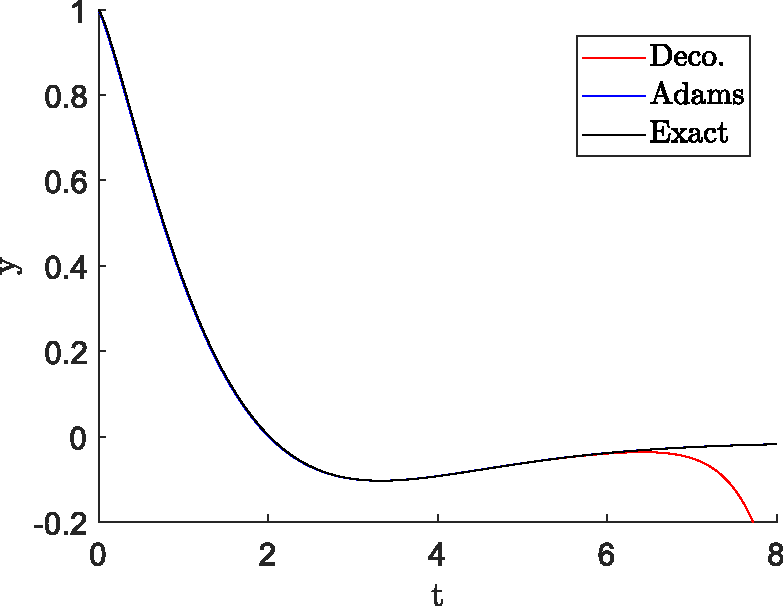
\includegraphics[scale=0.5]{files/adams_exact_deco.pdf}
    \caption{Results using ABM and decomposition}
    \label{fig:abm_decomp}
\end{figure}


OTROOOOOOOOOOOOOOOOOOOOOOOOOOOOOOOOOOOOOOOOOOOOOOOOOOOOOOOOOOOOOOOOOOOOOOOOOOOOOO EJEMPLOOOOOOOOOOOOOOOOOOOOOOOOOOOOOOOOOOOOOOOOOOOOOOOO
